\documentclass{beamer}
\usepackage{math214}
\usepackage{babel}

%\usepackage{enumitem}
% Then, after \begin{document}, you can begin your frames/slides

\title{\LARGE 255RC10}
\author{ Li Mingrui, Xia Yiwei, Zhang Haoran, Huang Jiayue}
\date{Summer 2024}

\definecolor{darkblue}{HTML}{6666dd} 
\colortheme{green!30!black}
%\colortheme{orange!85!black}
%\colortheme{darkblue}
%\colortheme{blue!100!black}
%\colortheme{orange!85!white!90!black}
\begin{document}

\maketitle



\begin{frame}{Contents}
    \begin{enumerate}
        \item \hyperlink{1}{Curl and Divergence}
        \item \hyperlink{2}{Parametric Surfaces and Areas}
        \item \hyperlink{3}{Surface Integrals}
    \end{enumerate}
       
\end{frame}

\section{Three Theorems}
    \begin{frame}{Conservative field}
        For a 3-D vector field $F=Pdx+Qdy+Rdz$, the 5 followings are equivalent:\\
        1. It is a conservative field\\
        2. $\forall$ piecewise smooth close curve $\mathcal{L}$, $\oint_{\mathcal{L}}F=0 $\\
        3.$\forall$ piecewise smooth curve $\mathcal{L'}$, $\int_{\mathcal{L}}F$ is path independent\\
        4. $\exists u$ s.t. $du=F$\\
        5.$\frac{\partial Q}{\partial x}=\frac{\partial P}{\partial y}, \frac{\partial Q}{\partial z}=\frac{\partial R}{\partial y}, \frac{\partial R}{\partial x}=\frac{\partial P}{\partial z}$
    \end{frame}
    \begin{frame}[t]{Green's Theorem}
        \begin{block}{}
            \par \textcolor{yy}{Definition.} Let $\mathcal{C}$ be a simple closed curve described by $\bar{r}: [a,b] \to \mathbb{R}^2$. We say that $\mathcal{C}$ is \textcolor{yy}{positively oriented} and call $\bar{r}$ a \textcolor{yy}{positive oriention of $\mathcal{C}$} if $\bar{r}(t)$ moves anticlockwise around $\mathcal{C}$ as $t$ ranges from $a$ to $b$.
        \end{block}

        \phantom{yy}

        \par \textcolor{yy}{Remark.} We use the symbols $\displaystyle \oint$ to denote such integrals.

        \phantom{yy}

        \par \textcolor{yy}{Theorem. (Green's Theorem)} Let $\mathcal{C}$ be a positively oriented, piecewise-smooth, simple closed curve in $\mathbb{R}^2$ and let $\mathcal{R}$ be the region enclosed by $\mathcal{C}$. Let $D \subset \mathbb{R}^2$ be an open region that contains $\mathcal{R}$. If $P: D \to \mathbb{R}$ and $Q: D \to \mathbb{R}$ have continuous partial derivatives on $D$, then 
        \begin{equation*}
            \int_{\mathcal{C}} Pdx + Qdy = \iint_{\mathcal{R}} \left( \dfrac{\partial Q}{\partial x} - \dfrac{\partial P}{\partial y}\right) dA.
        \end{equation*}
    \end{frame} 


\begin{frame}{Exercise of Green's Theorem}
    \begin{enumerate}
        \item $\oint_C(x+y) \mathrm{d} x-(x-y) \mathrm{d} y$, C is the oval $\dfrac{x^2}{a^2}+\dfrac{y^2}{b^2} = 1$, positively oriented.
        \item $P(x, y)=-\frac{y}{x^2+y^2}, Q(x, y)=\frac{x}{x^2+y^2}$ ,closed curve 
        $C:\left\{\begin{array}{l}x=2 \cos t, \\ y=3 \sin t\end{array} \quad 0 \leq t \leq 2 \pi $, 
        calculate $\oint_C P \mathrm{~d} x+Q \mathrm{~d} y$
    \end{enumerate}
\end{frame}



\begin{frame}{Stokes' Theorem}
        \par \textcolor{yy}{Theorem. (Stokes' Theorem)} Let $\mathcal{C}$ be a positively oriented, piecewise-smooth, simple, closed curve in $\mathbb{R}^3$ and let $\mathcal{S}$ be a surface whose boundary is $\mathcal{C}$ oriented with respect to the orientation of $\mathcal{C}$ according to the right-hand rule. Let $\bar{F}$ be a vector field on $\mathbb{R}^3$ whose component have continuous partial derivatives on a domain that contains $\mathcal{S}$, then 
        \begin{equation*}
            \int_{\mathcal{C}} \bar{F} \cdot d \bar{r} = \iint_{\mathcal{S}} \operatorname{curl}(\bar{F}) \cdot d \bar{S}.
        \end{equation*}
    \end{frame}

 


    \begin{frame}{Stokes' Theorem}
        \par In general, if $\mathcal{S}_1$ and $\mathcal{S}_2$ are oriented surfaces with the same oriented boundary curve $\mathcal{C}$ and both satisfy the hypotheses of Stokes' Theorem, then 
        \begin{equation*}
            \iint_{\mathcal{S}_1} \operatorname{curl}(\bar{F}) \cdot d \bar{S} = \int_{\mathcal{C}} \bar{F} \cdot d \bar{r} = \iint_{\mathcal{S}_2} \operatorname{curl}(\bar{F}) \cdot d \bar{S}
        \end{equation*}
    \end{frame}



    \begin{frame}{Exercise of Stokes' Theorem}
    Let C be the closed curve illustrated below
    \begin{figure}[H]
        \centering
        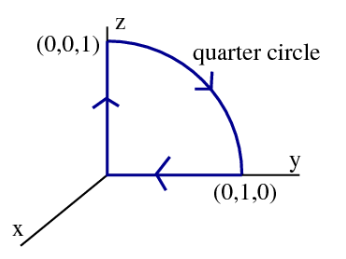
\includegraphics[width=0.5\linewidth]{1.png}
    
        \label{fig:1}
    \end{figure}
        For $F(x, y, z) = (y, z, x)$, compute $\int_C F\cdot ds$
    \end{frame}

    \begin{frame}{Divergence Theorem}
        \par \textcolor{yy}{Theorem. (Divergence Theorem)} Let $\mathcal{S}$ be a piecewise-smooth surface that encloses a solid $\mathcal{R}$ that is oriented so that the normal vectors point away from the interior of $\mathcal{S}$. Let $F$ be a vector field on $\mathbb{R}^3$ whose components have continuous partial derivatives on an open region that contains $\mathcal{R}$. Then 
        \begin{equation*}
            \iint_{\mathcal{S}} \bar{F} \cdot d\bar{S} = \iiint_{\mathcal{R}} \operatorname{div}(\bar{F}) dV.
        \end{equation*}
    \end{frame}


    \begin{frame}{Exercise of Divergence Theorem}
    Calculate $\iint_I=\frac{x}{r^3}dydz+\frac{y}{r^3}dxdz+\frac{z}{r^3}dxdy$, where $r=\sqrt{x^2+y^2+z^2}$, and S is:\\  
        (1) the outside of the ball $x^2+y^2+z^2=a^2$\\
        (2) the outside of the ball $(x-114)^2+(y-514)^2+(z-1919)^2=810^2$\\
        (3) the upper side of the surface $1-\frac{z}{7}=\frac{(x-2)^2}{25}+\frac{(y-1)^2}{16}$, where $z\geq 0$
        
    \end{frame}

    \begin{frame}{Summary}
    Green's Theorem\\
        \begin{equation*}
            \int_{\mathcal{C}} Pdx + Qdy = \iint_{\mathcal{R}} \left( \dfrac{\partial Q}{\partial x} - \dfrac{\partial P}{\partial y}\right) dA.
        \end{equation*}
        Stokes' Theorem\\
        \begin{equation*}
            \iint_{\mathcal{S}_1} \operatorname{curl}(\bar{F}) \cdot d \bar{S} = \int_{\mathcal{C}} \bar{F} \cdot d \bar{r}
        \end{equation*}
        Divergence Theorem\\
        \begin{equation*}
            \iint_{\mathcal{S}} \bar{F} \cdot d\bar{S} = \iiint_{\mathcal{R}} \operatorname{div}(\bar{F}) dV.
        \end{equation*}
        2D Divergence Theorem\\
        \begin{equation*}
            \int_{\mathcal{C}} \bar{F} \cdot\bar{n} ds = \iint_{\mathcal{R}} \operatorname{div}(\bar{F}) dA.
        \end{equation*}
    \end{frame}




\end{document}

